% Provenance (never printed): see sources/outline_sources.md (Year 2: radiogenic tracers
% Sr, Nd, Pb and mantle reservoirs; crustal growth; stable isotopes, delta notation and
% fractionation, d18O and d13C). Curves from figdata/bachelor-2/isotopes.py; exercise and
% problem values in the Book 4 scratch calculators calc/ch04.py and calc/ch04pb.py.
% Ruling (Sync 2): delta value and fractionation factor are chemistry's (Year 3 volume),
% recalled; this chapter defines the reference standards and the meteoric water line.
\chapter{Géochimie isotopique}\label{ch:b2:isotope-geochemistry}

Mangaia, dans le Pacifique sud, et Tristan da Cunha, dans l'Atlantique sud,
sont deux îles volcaniques bâties de basalte, et un échantillon de roche de l'une
ressemble beaucoup à un échantillon de l'autre, ou d'une dorsale médio-océanique.
Leurs isotopes les distinguent. Le strontium des basaltes de Mangaia porte la même
proportion de strontium-87 que celui des dorsales, soit environ
$^{87}\mathrm{Sr}/^{86}\mathrm{Sr} = 0.7028$, tandis que leur plomb compte parmi les plus
radiogéniques de la Terre, avec $^{206}\mathrm{Pb}/^{204}\mathrm{Pb}$ voisin de 21.6, contre
18.4 pour les dorsales. Les basaltes de Tristan contiennent davantage de strontium-87, de 0.7050 à
0.7054, et moins de néodyme-143 que l'un ou l'autre. La fusion ne trie pas les isotopes de ces
éléments lourds~: chaque lave porte donc la signature isotopique du manteau qui l'a fondu.
Le manteau terrestre n'est pas un réservoir unique mais plusieurs, qui ont conservé pendant des
milliards d'années des rapports parent--fils différents. Ce chapitre utilise la désintégration
radioactive du rubidium, du samarium, de l'uranium
et du thorium comme série de traceurs, suit l'évolution du manteau et de la croûte
continentale grâce aux isotopes du néodyme, sépare le manteau en réservoirs et en
mélanges de réservoirs, examine la vitesse de croissance des continents,
et se termine par les isotopes stables légers de l'oxygène, de l'hydrogène et du carbone, qui
tracent l'eau et le carbone à travers la Terre.
% ledger: data:b4-oib-isotopes, gale13:isotopes

\begin{recall}
Un parent radioactif se désintègre au taux $\lambda P$, et dans un système fermé le
rapport du fils croît selon $(D/D_s)_{\text{actuel}} = (D/D_s)_0 + (P/D_s)_{\text{actuel}}
(e^{\lambda t}-1)$, $D_s$ étant un isotope stable du fils~; des minéraux ou des
roches formés ensemble se placent sur une isochrone, dont la pente donne l'âge et dont
l'ordonnée à l'origine donne le rapport initial (volume de lycée, dernière année~; volume de
première année, chapitre sur la datation radiométrique). Un spectromètre de masse sépare les ions selon leur
rapport masse sur charge (volume de chimie de deuxième année). La valeur $\delta$ d'un
échantillon est $\delta = (R_{\text{échantillon}}/R_{\text{étalon}} - 1)\times 1000$, en pour
mille, et le facteur de fractionnement entre deux phases A et B est
$\alpha_{\mathrm{A/B}} = R_{\mathrm A}/R_{\mathrm B}$, $R$ étant le rapport de l'isotope
lourd à l'isotope léger~; ces deux grandeurs sont introduites, avec les énergies de point zéro
qui causent le fractionnement isotopique, dans le volume de chimie de troisième année.
Les \omterm{def:b2:elements-in-the-earth:partition}{éléments incompatibles}, le MORB et l'OIB ont été définis au
\cref{ch:b2:elements-in-the-earth}.
\end{recall}

\section{Traceurs isotopiques radiogéniques}

Trois systèmes de désintégration portent l'essentiel de l'information sur le manteau et la croûte.
Le rubidium-87 se désintègre en strontium-87, le samarium-147 en néodyme-143, et l'uranium
et le thorium, par leurs chaînes de désintégration, en trois isotopes du plomb. Chaque parent
et chaque fils se comportent différemment lors de la fusion, et chaque fils possède un
isotope stable non radiogénique par rapport auquel il est mesuré.

\begin{table}[ht]
\centering
\begin{tabular}{lllll}
\hline
parent & fils & rapport mesuré & constante de désintégration (par an) & demi-vie (Ga)\\
\hline
$^{87}$Rb & $^{87}$Sr & $^{87}\mathrm{Sr}/^{86}\mathrm{Sr}$ & \num{1.3972e-11} & 49.6\\
$^{147}$Sm & $^{143}$Nd & $^{143}\mathrm{Nd}/^{144}\mathrm{Nd}$ & \num{6.524e-12} & 106.25\\
$^{238}$U & $^{206}$Pb & $^{206}\mathrm{Pb}/^{204}\mathrm{Pb}$ & \num{1.55125e-10} & 4.47\\
\hline
\end{tabular}
\caption{Trois systèmes de désintégration à longue durée de vie utilisés comme traceurs. Données~:
recommandations IUPAC--IUGS (Villa et al., 2020 et 2022).}
\label{tab:b2:isotope-geochemistry:decay}
\end{table}
% ledger: villa22:rb87, villa20:sm147

\begin{definition}[Traceur isotopique radiogénique]\label{def:b2:isotope-geochemistry:tracer}
Un \emph{traceur isotopique radiogénique}\index{traceur isotopique radiogénique} est le rapport
d'un isotope fils produit par un parent radioactif à longue durée de vie à un
isotope stable du même élément, tel que $^{87}\mathrm{Sr}/^{86}\mathrm{Sr}$ ou
$^{143}\mathrm{Nd}/^{144}\mathrm{Nd}$, utilisé pour identifier la source d'une roche plutôt
que pour la dater. Le rapport d'un réservoir croît à une vitesse fixée par son
rapport parent--fils, et enregistre ainsi l'histoire de ce rapport.
\end{definition}

Les deux éléments d'un couple de désintégration sont séparés dès que le manteau fond. Au
\cref{ch:b2:elements-in-the-earth}, le rubidium s'est révélé plus incompatible que
le strontium, et le néodyme plus incompatible que le samarium. Une fusion, et la croûte
qu'elle construit, laisse donc le manteau avec un Rb/Sr élevé et un Sm/Nd faible~;
le résidu conserve un Rb/Sr faible et un Sm/Nd élevé. Au fil du temps, la croûte
accumule du strontium-87 plus vite que sa source et du néodyme-143 plus lentement~;
le \omterm{def:b2:isotope-geochemistry:reservoirs}{manteau appauvri} fait l'inverse. Les rapports des deux couples évoluent
en sens opposés, un point que le diagramme Sr--Nd ci-dessous rend évident.

\begin{proposition}[Les rapports isotopiques survivent à la fusion]\label{prop:b2:isotope-geochemistry:melting}
Lorsqu'une roche fond et que le liquide se sépare du résidu, les
rapports $^{87}\mathrm{Sr}/^{86}\mathrm{Sr}$ et $^{143}\mathrm{Nd}/^{144}\mathrm{Nd}$ du liquide
égalent ceux de la source à la précision des mesures près~;
seuls les rapports parent--fils, Rb/Sr et Sm/Nd, sont modifiés.
\end{proposition}
\admitted

\noindent L'énoncé repose sur deux faits. Les isotopes d'un même élément ont la
même structure électronique~: ils entrent donc presque également dans un cristal ou dans un liquide~; la
différence de masse relative entre le strontium-87 et le strontium-86, environ un pour
cent, est bien plus faible que pour l'oxygène ou l'hydrogène, et à haute température le
logarithme d'un facteur de fractionnement à l'équilibre décroît comme l'inverse du carré de
la température, vers 1. Par ailleurs la mesure elle-même corrige le fractionnement
qui se produit dans le spectromètre de masse, en fixant le rapport de deux isotopes
non radiogéniques (pour le néodyme, $^{146}\mathrm{Nd}/^{144}\mathrm{Nd} =
0.7219$), ce qui effacerait aussi tout fractionnement naturel faible. Une lave
échantillonne donc les rapports isotopiques de sa source, tandis que ses rapports
d'\omterm{def:b2:elements-in-the-earth:trace}{éléments en traces} reflètent aussi la fusion.
% ledger: white:chur, white:t-dependence

\section{L'évolution du manteau et de la croûte}

\subsection{Le réservoir chondritique}

Le samarium et le néodyme sont tous deux des \omterm{def:b2:elements-in-the-earth:ree}{terres rares} lithophiles réfractaires
(\cref{ch:b2:elements-in-the-earth})~: la \omterm{def:b2:elements-in-the-earth:bse}{Terre silicatée globale} devrait avoir conservé leur
rapport chondritique. Les \omterm{def:b2:planet-formation-meteorites:chondrule}{chondrites} donnent alors l'histoire Sm--Nd de la Terre
non différenciée.

\begin{definition}[Réservoir uniforme chondritique]\label{def:b2:isotope-geochemistry:chur}
Le \emph{réservoir uniforme chondritique}\index{réservoir uniforme chondritique}
(CHUR) est un réservoir modèle ayant la composition samarium--néodyme des \omterm{def:b2:planet-formation-meteorites:chondrule}{chondrites},
fermé depuis la formation du Système solaire. Ses rapports actuels sont
$(^{143}\mathrm{Nd}/^{144}\mathrm{Nd})_{\mathrm{CHUR}} = 0.512638$ et
$(^{147}\mathrm{Sm}/^{144}\mathrm{Nd})_{\mathrm{CHUR}} = 0.1966$.
\end{definition}
% ledger: white:chur

En remontant le temps avec l'équation de l'isochrone, le CHUR avait, lorsque les premiers solides se sont condensés il y a
\qty{4567}{Ma} (\cref{ch:b2:planet-formation-meteorites}),
\[
  ^{143}\mathrm{Nd}/^{144}\mathrm{Nd} = 0.512638 - 0.1966\,\bigl(e^{\lambda\cdot
  \num{4.567e9}\,\mathrm{an}}-1\bigr) = 0.506692 .
\] Depuis, son rapport a augmenté de
1.2 pour cent. Les différences entre roches terrestres sont mille fois
plus petites, et s'expriment dans une unité plus commode.
% ledger: lugaro:cai, villa20:sm147

\begin{definition}[Notation epsilon]\label{def:b2:isotope-geochemistry:epsilon}
La \emph{notation epsilon}\index{notation epsilon} exprime le
rapport $^{143}\mathrm{Nd}/^{144}\mathrm{Nd}$ d'un échantillon, à un instant $t$ avant le
présent, comme son écart relatif au CHUR à la même date, en parties pour dix
mille~:
\[
  \varepsilon_{\mathrm{Nd}}(t) = \left(
  \frac{(^{143}\mathrm{Nd}/^{144}\mathrm{Nd})_{\text{échantillon}}(t)}
       {(^{143}\mathrm{Nd}/^{144}\mathrm{Nd})_{\mathrm{CHUR}}(t)} - 1\right)\times 10^4 .
\]
Sans date, $\varepsilon_{\mathrm{Nd}}$ est la valeur actuelle.
\end{definition}

Le MORB moyen, avec $^{143}\mathrm{Nd}/^{144}\mathrm{Nd} = 0.513074$, a
$\varepsilon_{\mathrm{Nd}} = (0.513074/0.512638 - 1)\times10^4 = +8.5$~; la plupart des roches
se situent entre $-20$ et $+10$. Une valeur positive signifie que la source de la roche a eu,
en moyenne au cours de l'histoire de la Terre, un Sm/Nd plus élevé que celui des \omterm{def:b2:planet-formation-meteorites:chondrule}{chondrites}~:
elle est appauvrie en l'élément le plus incompatible, le néodyme. Une valeur négative signifie
l'inverse. L'écart au Sm/Nd chondritique se mesure par la
déviation fractionnaire
\[
  f_{\mathrm{Sm/Nd}} = \frac{(\mathrm{Sm}/\mathrm{Nd})_{\text{échantillon}}}
  {(\mathrm{Sm}/\mathrm{Nd})_{\mathrm{CHUR}}} - 1,
\]
qui ne dépend pas de savoir si les rapports sont massiques ou atomiques. Avec les valeurs CI
du \cref{ch:b2:elements-in-the-earth} (Sm 0.145, Nd \qty{0.457}{ppm},
$\mathrm{Sm}/\mathrm{Nd} = 0.317$), la croûte continentale supérieure (4.7 et
\qty{27}{ppm}, 0.174) a $f_{\mathrm{Sm/Nd}} = -0.45$.
% ledger: gale13:isotopes, white:chur, lodders:ci-table, rg03:ucc-trace

\begin{proposition}[Croissance linéaire de $\varepsilon_{\mathrm{Nd}}$]\label{prop:b2:isotope-geochemistry:linear}
Un réservoir séparé du CHUR et ayant conservé depuis lors la déviation fractionnaire
$f_{\mathrm{Sm/Nd}}$ voit son $\varepsilon_{\mathrm{Nd}}$ évoluer vers l'avant
dans le temps, au taux
\[
  \frac{\mathrm{d}\varepsilon_{\mathrm{Nd}}}{\mathrm{d}\tau} \approx Q\,f_{\mathrm{Sm/Nd}},
  \qquad
  Q = 10^4\,\lambda_{147}\,
  \frac{(^{147}\mathrm{Sm}/^{144}\mathrm{Nd})_{\mathrm{CHUR}}}
       {(^{143}\mathrm{Nd}/^{144}\mathrm{Nd})_{\mathrm{CHUR}}}
  = \qty{25.0}{\per\Ga},
\]
où $\tau$ est le temps compté vers l'avant. Un réservoir ayant $\varepsilon_0$ au moment de sa
séparation, il y a un temps $T$, a aujourd'hui $\varepsilon_{\mathrm{Nd}} \approx \varepsilon_0
+ Q f_{\mathrm{Sm/Nd}} T$.
\end{proposition}

\begin{proof}
Notons $R$ le rapport $^{143}\mathrm{Nd}/^{144}\mathrm{Nd}$ et $p$ le rapport
$^{147}\mathrm{Sm}/^{144}\mathrm{Nd}$. Dans un réservoir fermé
$\mathrm{d}R/\mathrm{d}\tau = \lambda p\,e^{\lambda t}$, avec $t$ le temps avant le
présent~; car $\lambda t \le 0.03$, le facteur $e^{\lambda t}$ diffère de 1 d'au
plus 3 pour cent, et $\mathrm{d}R/\mathrm{d}\tau \approx \lambda p$. Alors
$\mathrm{d}(R_s - R_c)/\mathrm{d}\tau \approx \lambda (p_s - p_c) = \lambda p_c
f_{\mathrm{Sm/Nd}}$, car $p_s/p_c - 1 = f_{\mathrm{Sm/Nd}}$. Divisant par $R_c$,
qui ne change que de 1.2 pour cent sur l'âge de la Terre, on obtient
$\mathrm{d}\varepsilon/\mathrm{d}\tau \approx 10^4\lambda p_c f/R_c$. Avec
$\lambda = \qty{6.524e-12}{\per\year}$, $p_c = 0.1966$ et $R_c = 0.512638$, $Q =
\num{2.502e-8}$ par an, soit \qty{25.0}{\per\Ga}.
\end{proof}
% ledger: villa20:sm147, white:chur

Une croûte ayant le Sm/Nd de la croûte supérieure ($f = -0.45$) perd donc environ
11 unités epsilon par milliard d'années par rapport au CHUR, tandis qu'un réservoir mantellique
n'a besoin que de $f = +0.07$ pour passer de 0 à la valeur MORB de $+8.5$ en
\qty{4.567}{Ga}. La figure ci-dessous suit les équations exactes pour trois
réservoirs~: le CHUR, un \omterm{def:b2:isotope-geochemistry:reservoirs}{manteau appauvri} fermé depuis la formation de la Terre avec le Sm/Nd
qui l'amène à la valeur MORB aujourd'hui ($^{147}\mathrm{Sm}/^{144}\mathrm{Nd} =
0.211$), et une croûte extraite de ce manteau il y a 2.7 milliards d'années avec le Sm/Nd de la
croûte continentale supérieure ($0.108$). La croûte partait de $\varepsilon_{\mathrm{Nd}} =
+3.5$, valeur de sa source à cette époque, et se situe aujourd'hui à $-27$.

\begin{definition}[Manteau appauvri, manteau enrichi]\label{def:b2:isotope-geochemistry:reservoirs}
Un \emph{manteau appauvri}\index{manteau appauvri} est une partie du manteau
ayant cédé des \omterm{def:b2:elements-in-the-earth:partition}{éléments incompatibles} à des liquides, de sorte que son Sm/Nd est plus élevé et son Rb/Sr
plus bas que celui des \omterm{def:b2:planet-formation-meteorites:chondrule}{chondrites}~; avec le temps son $\varepsilon_{\mathrm{Nd}}$ devient positif et
son $^{87}\mathrm{Sr}/^{86}\mathrm{Sr}$ faible. Un \emph{manteau
enrichi}\index{manteau enrichi} est une partie du manteau qui a gagné
des \omterm{def:b2:elements-in-the-earth:partition}{éléments incompatibles}, par exemple à partir de croûte recyclée ou de petits liquides de fusion,
avec un $\varepsilon_{\mathrm{Nd}}$ négatif ou un $^{87}\mathrm{Sr}/^{86}\mathrm{Sr}$ élevé.
\end{definition}

\begin{omfigure}
\centering
\begin{tikzpicture}
\begin{axis}[omrecord, width=0.82\linewidth, height=6.4cm,
  x dir=reverse, xmin=0, xmax=4.6, ymin=-30, ymax=12,
  xlabel={temps avant le présent (Ga)}, ylabel={$\varepsilon_{\mathrm{Nd}}(t)$},
  tick label style={font=\scriptsize}, label style={font=\small}]
\addplot[thick, black] table[x=t_Ga, y=eps] {figdata/out/bachelor-2-isotopes-chur.dat};
\addplot[very thick, blue!70!black] table[x=t_Ga, y=eps] {figdata/out/bachelor-2-isotopes-dm.dat};
\addplot[very thick, brown!70!black] table[x=t_Ga, y=eps] {figdata/out/bachelor-2-isotopes-crust.dat};
\addplot[densely dashed, gray] coordinates {(2.7,-30) (2.7,12)};
\node[font=\scriptsize, anchor=north] at (axis cs:3.6,-0.6) {CHUR};
\node[font=\scriptsize, blue!70!black, anchor=south east] at (axis cs:0.4,8.8) {manteau appauvri, $+8.5$};
\node[font=\scriptsize, brown!70!black, anchor=north east] at (axis cs:0.3,-25.5) {croûte, $-27$};
\node[font=\scriptsize, gray, anchor=north west, align=left] at (axis cs:2.65,-12) {croûte extraite\\à \qty{2.7}{Ga}};
\end{axis}
\end{tikzpicture}
\par\smallskip{\small Évolution isotopique du néodyme, en $\varepsilon_{\mathrm{Nd}}$, du
réservoir chondritique (nul par définition), d'un \omterm{def:b2:isotope-geochemistry:reservoirs}{manteau appauvri} fermé depuis
\qty{4.567}{Ga} dont le Sm/Nd amène le MORB moyen actuel, et d'une croûte
extraite de celui-ci il y a \qty{2.7}{Ga} avec le Sm/Nd de la croûte continentale
supérieure. Chaque droite est presque rectiligne, comme l'affirme la proposition de croissance linéaire. Données~:
CHUR, texte de White~; MORB moyen, Gale et al. (2013)~; Sm/Nd de la croûte,
Rudnick et Gao.}
\end{omfigure}
% ledger: white:chur, villa20:sm147, gale13:isotopes, rg03:ucc-trace, lodders:ci-table, lugaro:cai

\subsection{Deux réservoirs complémentaires}

Si la croûte continentale et le \omterm{def:b2:isotope-geochemistry:reservoirs}{manteau appauvri} provenaient d'un même réservoir chondritique,
leur néodyme doit se recomposer en la valeur chondritique. Le néodyme est
le vecteur~: chaque réservoir compte en proportion du néodyme qu'il contient.

\begin{proposition}[Bilan de masse isotopique]\label{prop:b2:isotope-geochemistry:mass-balance}
Soient des réservoirs $i$ de masses $M_i$ et de concentrations en néodyme $C_i$ issus
de la division d'un même réservoir parent. Alors, à très bonne approximation,
\[
  \sum_i M_i C_i\, \varepsilon_i = \Bigl(\sum_i M_i C_i\Bigr) \varepsilon_{\text{parent}},
\]
les deux membres étant évalués au même instant, et le parent étant suivi comme s'il
était resté entier.
\end{proposition}

\begin{proof}
Le nombre d'atomes de $^{143}\mathrm{Nd}$ et celui des atomes de $^{144}\mathrm{Nd}$
se conservent chacun lors de la division, et chacun croît (pour
$^{143}\mathrm{Nd}$) ou reste constant (pour $^{144}\mathrm{Nd}$) dans chaque réservoir
exactement comme dans le tout. D'où la moyenne, pondérée par le $^{144}\mathrm{Nd}$, des rapports $R_i$
égale le rapport du parent, $R_p$. La part du $^{144}\mathrm{Nd}$
dans le néodyme varie entre réservoirs de bien moins d'un millième, de sorte que
pondérer par $M_iC_i$ revient à pondérer par le $^{144}\mathrm{Nd}$. Enfin $\varepsilon$ est une
fonction linéaire de $R$ à un instant donné, $\varepsilon = 10^4(R/R_c - 1)$, et une
moyenne pondérée de fonctions linéaires est la fonction linéaire de la moyenne pondérée.
\end{proof}

Avec la valeur de la croûte supérieure, \qty{27}{ppm} de néodyme, prise pour toute la
croûte, une croûte continentale de \qty{7.2e9}{km^3} à \qty{2830}{kg/m^3}, soit
\qty{2.0e22}{kg} ou 0.51 pour cent de la masse de la Terre silicatée, contient
$0.0051\times27/1.25 = 11$ pour cent du néodyme de la Terre silicatée (\omterm{def:b2:elements-in-the-earth:bse}{manteau primitif},
\qty{1.25}{ppm}). Si la croûte a un $\varepsilon_{\mathrm{Nd}}$ moyen de
$-15$, une contribution négative de $0.11\times15 = 1.65$ unité doit être
compensée par le manteau~: un réservoir à la valeur MORB de $+8.5$ devrait contenir
environ un cinquième du néodyme de la Terre silicatée (voir l'\cref{exo:b2:isotope-geochemistry:9}). C'est l'un des
arguments selon lesquels le \omterm{def:b2:isotope-geochemistry:reservoirs}{manteau appauvri} échantillonné par les dorsales n'est pas l'ensemble du
manteau.
% ledger: cogley84:continents, cm95:crust, ms95:pm-trace, rg03:ucc-trace, data:prem, earth:mass, gale13:isotopes

\section{Les réservoirs du manteau}

Les rapports isotopiques des basaltes océaniques échantillonnent le manteau sans traverser
la croûte continentale. Tracés l'un contre l'autre, ils montrent à la fois la
complémentarité de la croûte et du \omterm{def:b2:isotope-geochemistry:reservoirs}{manteau appauvri}, ainsi que l'existence d'autres
réservoirs.

Les isotopes du strontium et du néodyme sont anticorrélés dans la plupart des basaltes
océaniques~: une lave à $\varepsilon_{\mathrm{Nd}}$ élevé a un faible
$^{87}\mathrm{Sr}/^{86}\mathrm{Sr}$. Cette bande est appelée bande mantellique~; elle découle du
comportement opposé des deux couples lors de la fusion (le rubidium moins
compatible que le strontium, le samarium plus compatible que le néodyme). Le MORB moyen
se situe à son extrémité appauvrie, avec $^{87}\mathrm{Sr}/^{86}\mathrm{Sr} = 0.702819$ et
$\varepsilon_{\mathrm{Nd}} = +8.5$. Les \omterm{def:b2:elements-in-the-earth:morb-oib}{basaltes d'île océanique} s'étalent à partir de là vers
des $\varepsilon_{\mathrm{Nd}}$ plus bas et des $^{87}\mathrm{Sr}/^{86}\mathrm{Sr}$ plus élevés, mais pas
le long d'une seule droite.
% ledger: white:dm, gale13:isotopes

\begin{definition}[Pôle mantellique]\label{def:b2:isotope-geochemistry:end-members}
Un \emph{pôle mantellique}\index{pôle mantellique} est l'une des compositions isotopiques extrêmes
à partir desquelles les rapports isotopiques du Sr, du Nd et du Pb des basaltes océaniques peuvent être
construits par mélange. Quatre sont couramment nommés~: DMM, le manteau MORB
appauvri (faible $^{87}\mathrm{Sr}/^{86}\mathrm{Sr}$, $\varepsilon_{\mathrm{Nd}}$ élevé)~;
HIMU, pour un $\mu = {}^{238}\mathrm{U}/^{204}\mathrm{Pb}$ élevé dans sa source
(plomb très radiogénique, $^{206}\mathrm{Pb}/^{204}\mathrm{Pb}$ supérieur à 20, avec un faible
$^{87}\mathrm{Sr}/^{86}\mathrm{Sr}$)~; EM1, \omterm{def:b2:isotope-geochemistry:reservoirs}{manteau enrichi} 1 (assez fort
$^{87}\mathrm{Sr}/^{86}\mathrm{Sr}$, $\varepsilon_{\mathrm{Nd}}$ négatif, plomb
peu radiogénique)~; et EM2, \omterm{def:b2:isotope-geochemistry:reservoirs}{manteau enrichi} 2 (fort $^{87}\mathrm{Sr}/^{86}\mathrm{Sr}$).
\end{definition}
% ledger: white:end-members

\begin{omfigure}
\centering
\begin{tikzpicture}
\begin{axis}[omrecord, width=0.82\linewidth, height=6.6cm,
  xmin=0.7020, xmax=0.7064, ymin=-6, ymax=11,
  xlabel={$^{87}\mathrm{Sr}/^{86}\mathrm{Sr}$}, ylabel={$\varepsilon_{\mathrm{Nd}}$},
  xticklabel style={/pgf/number format/fixed, /pgf/number format/precision=4},
  scaled x ticks=false, legend pos=south west, legend cell align=left,
  legend style={font=\scriptsize}, tick label style={font=\scriptsize},
  label style={font=\small}]
\addplot[only marks, mark=*, mark size=1.3pt, red!70!black] table[x=sr, y=eps] {figdata/out/bachelor-2-isotopes-himu.dat};
\addlegendentry{type HIMU~: St.\ Helena, Mangaia, Tubuai}
\addplot[only marks, mark=square*, mark size=1.2pt, brown!70!black] table[x=sr, y=eps] {figdata/out/bachelor-2-isotopes-em1.dat};
\addlegendentry{type EM1~: Tristan da Cunha, Gough}
\addplot[only marks, mark=diamond*, mark size=3pt, blue!70!black] table[x=sr, y=eps] {figdata/out/bachelor-2-isotopes-morb.dat};
\addlegendentry{MORB moyen}
\addplot[densely dashed, gray] coordinates {(0.7020,0) (0.7064,0)};
\node[font=\scriptsize, gray, anchor=south east] at (axis cs:0.7063,0.1) {CHUR};
\draw[->, gray] (axis cs:0.7030,9.5) -- (axis cs:0.7046,0.8);
\node[font=\scriptsize, gray, anchor=west, align=left] at (axis cs:0.7036,6.5) {la bande mantellique~:\\appauvri vers enrichi};
\end{axis}
\end{tikzpicture}
\par\smallskip{\small Isotopes du strontium et du néodyme de 89 basaltes de cinq
îles océaniques et du basalte moyen de dorsale médio-océanique. Les îles de type HIMU se placent sous la
bande principale, avec le faible rapport du strontium du MORB mais un
$\varepsilon_{\mathrm{Nd}}$ plus bas~; les îles de type EM1 se situent du côté enrichi du CHUR.
Les laves samoanes de type EM2 atteignent $^{87}\mathrm{Sr}/^{86}\mathrm{Sr} = 0.7205$, bien
au-delà de cette échelle, vers la droite. Données~: Stracke et al. (2022), CC BY 4.0~; Gale et
al. (2013)~; Edwards et al. (2019).}
\end{omfigure}
% ledger: data:b4-oib-isotopes, gale13:isotopes, edwards19:samoa, white:chur

Les groupes d'îles de la figure ci-dessus ne sont pas quelconques. Le groupe de Sainte-Hélène,
qui comprend les îles Australes (Mangaia et Tubuai parmi elles) et l'Ascension,
se place sous la bande principale et possède le plomb le plus radiogénique
($^{206}\mathrm{Pb}/^{204}\mathrm{Pb}$ supérieur à 20~; Mangaia atteint 21.5 à 22.0). Le
groupe des Kerguelen, Tristan da Cunha, Gough et Kerguelen, se situe à un
$^{87}\mathrm{Sr}/^{86}\mathrm{Sr}$ assez élevé et à un $\varepsilon_{\mathrm{Nd}}$ négatif, toujours avec
un plomb peu radiogénique. Le groupe de la Société, avec Samoa et les Marquises, dessine une
tendance Sr--Nd moins pentue, atteignant des rapports du strontium très élevés~: deux laves samoanes
ont des $^{87}\mathrm{Sr}/^{86}\mathrm{Sr}$ de 0.7186 et 0.7205, supérieurs à
celui de l'eau de mer actuelle (0.7092). Les groupes de Sainte-Hélène, des Kerguelen et de la Société sont les types
HIMU, EM1 et EM2.
% ledger: white:end-members, data:b4-oib-isotopes, edwards19:samoa

Un rapport qui diffère entre deux parties du manteau a dû être maintenu par une différence
de rapport parent--fils pendant très longtemps~: un écart de 10 unités
d'$\varepsilon_{\mathrm{Nd}}$ exige, selon la proposition de croissance linéaire, 1 milliard d'années à $f = 0.4$
ou 4 milliards d'années à $f = 0.1$. Les réservoirs du manteau sont donc anciens.
Ce qu'ils sont se lit dans les rapports parent--fils que réclament leurs isotopes. HIMU exige
un U/Pb élevé et un Rb/Sr faible pendant longtemps, ce qui correspond à une croûte océanique
ayant perdu du plomb et du rubidium dans les fluides libérés au-dessus d'une zone de subduction,
puis stockée dans le manteau pendant un ou deux milliards d'années.
EM1 et EM2 exigent un Sm/Nd faible et, pour EM2, un Rb/Sr élevé~: la signature
d'un matériau issu des continents, tel qu'un sédiment recyclé, ou d'un \omterm{def:b2:isotope-geochemistry:reservoirs}{manteau enrichi}
par de petits liquides de fusion. Ces interprétations sont discutées~;
les mesures, elles, ne le sont pas.
% ledger: white:end-members

\begin{omfigure}
\centering
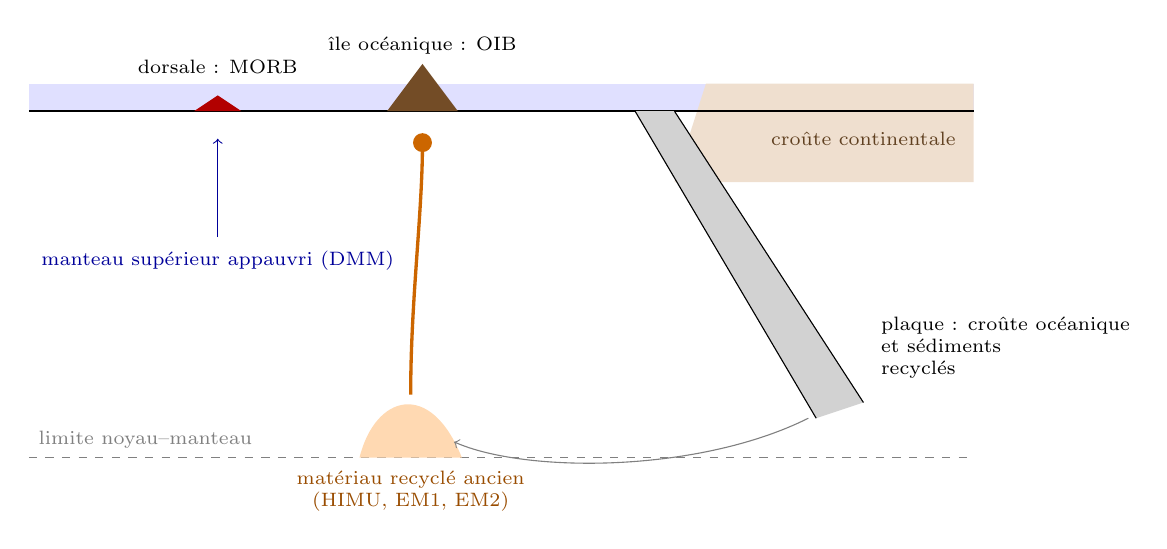
\begin{tikzpicture}[x=1cm, y=1cm, font=\scriptsize]
  % surface and lithosphere
  \fill[blue!12] (-6,0) rectangle (6,0.35);
  \fill[brown!25] (2.6,0.35) -- (6,0.35) -- (6,-0.9) -- (2.2,-0.9) -- cycle;
  \node[brown!50!black] at (4.6,-0.35) {croûte continentale};
  \draw[thick] (-6,0) -- (6,0);
  % ridge
  \node[anchor=south] at (-3.6,0.35) {dorsale~: MORB};
  \draw[->, blue!60!black] (-3.6,-1.6) -- (-3.6,-0.35);
  \node[blue!60!black, anchor=north] at (-3.6,-1.65) {manteau supérieur appauvri (DMM)};
  % slab
  \fill[gray!35] (1.7,0) -- (2.2,0) -- (4.6,-3.7) -- (4.0,-3.9) -- cycle;
  \draw (1.7,0) -- (4.0,-3.9) (2.2,0) -- (4.6,-3.7);
  \node[anchor=west, align=left] at (4.7,-3.0) {plaque~: croûte océanique\\et sédiments\\recyclés};
  % deep pool and plume
  \draw[gray, dashed] (-6,-4.4) -- (6,-4.4);
  \node[anchor=south west, gray] at (-6,-4.4) {limite noyau--manteau};
  \fill[orange!30] (-1.8,-4.4) .. controls (-1.6,-3.6) and (-0.9,-3.4) .. (-0.5,-4.4) -- cycle;
  \draw[very thick, orange!80!black] (-1.15,-3.6) .. controls (-1.15,-2.4) and (-1.0,-1.3) .. (-1.0,-0.4);
  \fill[orange!80!black] (-1.0,-0.4) circle (0.12);
  \fill[brown!60!black] (-1.45,0) -- (-1.0,0.6) -- (-0.55,0) -- cycle;
  \node[anchor=south] at (-1.0,0.6) {île océanique~: OIB};
  \fill[red!70!black] (-3.9,0) -- (-3.6,0.2) -- (-3.3,0) -- cycle;
  \node[orange!60!black, anchor=north, align=center] at (-1.15,-4.45) {matériau recyclé ancien\\(HIMU, EM1, EM2)};
  \draw[->, gray] (3.9,-3.9) .. controls (2.5,-4.6) and (0.3,-4.6) .. (-0.6,-4.2);
\end{tikzpicture}
\par\smallskip{\small Une interprétation largement utilisée des réservoirs du manteau, non à l'échelle~: les dorsales
échantillonnent le manteau supérieur appauvri~; la croûte océanique et les sédiments retournent
au manteau aux zones de subduction~; des panaches remontant du manteau profond ramènent des matériaux
où se mêlent d'anciennes composantes recyclées, et donnent aux îles leur caractère
HIMU, EM1 ou EM2.}
\end{omfigure}

\section{Mélange}

De nombreux ensembles isotopiques sont des mélanges. Une lave peut provenir d'une source qui est un
mélange de deux réservoirs, ou un magma peut incorporer une partie de la croûte qu'il traverse.
Les deux cas obéissent à la même algèbre.

\begin{proposition}[Hyperbole de mélange]\label{prop:b2:isotope-geochemistry:mixing}
Soit un mélange contenant une fraction massique $f$ du constituant A et $1-f$ du constituant
B. Pour un élément de concentrations $C_{\mathrm A}$, $C_{\mathrm B}$ et de rapports isotopiques
$R_{\mathrm A}$, $R_{\mathrm B}$~:
\begin{enumerate}
\item la concentration du mélange, $C = fC_{\mathrm A} + (1-f)C_{\mathrm B}$, et
son rapport isotopique,
$R = \bigl(fC_{\mathrm A}R_{\mathrm A} + (1-f)C_{\mathrm B}R_{\mathrm B}\bigr)/C$, satisfont
$R = a + b/C$ avec des constantes $a$ et $b$~: les mélanges se placent sur une droite dans
un tracé de $R$ en fonction de $1/C$~;
\item deux tels rapports de deux éléments, $R$ et $R'$, se placent sur une hyperbole, appelée
\emph{hyperbole de mélange}\index{hyperbole de mélange}, qui n'est une droite que
si le rapport des deux éléments est le même dans A et dans B. Sa courbure est fixée par
$K = (C'/C)_{\mathrm A}/(C'/C)_{\mathrm B}$.
\end{enumerate}
\end{proposition}

\begin{proof}
(1) Éliminons $f$~: $f = (C - C_{\mathrm B})/(C_{\mathrm A} - C_{\mathrm B})$. Alors
$RC = C_{\mathrm B}R_{\mathrm B} + f(C_{\mathrm A}R_{\mathrm A} - C_{\mathrm B}R_{\mathrm
B})$ est linéaire en $C$, $RC = \alpha + \beta C$, et $R = \beta + \alpha/C$.
(2) La part de l'élément qui provient de A est $s = fC_{\mathrm A}/C$, et $R =
R_{\mathrm B} + s(R_{\mathrm A} - R_{\mathrm B})$ est linéaire en $s$~; de même $R'$ est
linéaire en $s' = fC'_{\mathrm A}/C'$. Avec $u = f/(1-f)$, $s = u C_{\mathrm
A}/(uC_{\mathrm A} + C_{\mathrm B})$ et $s' = uC'_{\mathrm A}/(uC'_{\mathrm A} +
C'_{\mathrm B})$. Éliminer $u$ donne $s' = Ks/(1 + (K-1)s)$, une hyperbole dans le
plan $(s, s')$, donc dans le plan $(R, R')$~; c'est la droite $s' = s$
lorsque $K = 1$.
\end{proof}

\begin{omfigure}
\centering
\begin{tikzpicture}
\begin{axis}[omrecord, width=0.62\linewidth, height=6.2cm,
  xmin=0, xmax=1, ymin=0, ymax=1,
  xlabel={premier rapport, réduit (B $=0$, A $=1$)},
  ylabel={deuxième rapport, réduit},
  tick label style={font=\scriptsize}, label style={font=\small}]
\addplot[thick, red!70!black] table[x=x, y=y] {figdata/out/bachelor-2-isotopes-mixK50.dat};
\addplot[thick, black] table[x=x, y=y] {figdata/out/bachelor-2-isotopes-mixK10.dat};
\addplot[thick, blue!70!black] table[x=x, y=y] {figdata/out/bachelor-2-isotopes-mixK02.dat};
\node[font=\scriptsize, red!70!black, anchor=south east] at (axis cs:0.30,0.72) {$K=5$};
\node[font=\scriptsize, anchor=south east] at (axis cs:0.55,0.56) {$K=1$};
\node[font=\scriptsize, blue!70!black, anchor=north west] at (axis cs:0.62,0.22) {$K=0.2$};
\node[font=\scriptsize, anchor=north west] at (axis cs:0.0,0.0) {B};
\node[font=\scriptsize, anchor=south east] at (axis cs:1.0,1.0) {A};
\end{axis}
\end{tikzpicture}
\par\smallskip{\small Courbes de mélange entre deux constituants A et B pour trois
valeurs de $K$, rapport des deux éléments dans A divisé par celui de B. Chaque
rapport isotopique est réduit à 0 en B et à 1 en A~; le second élément est $K$ fois
plus riche en A, par rapport au premier, qu'en B, si bien que le second rapport se déplace vers
A plus vite lorsque $K > 1$.}
\end{omfigure}

Un constituant riche en un élément domine le rapport isotopique de cet élément dans le
mélange. Un sédiment recyclé contient des dizaines de fois plus de néodyme que le \omterm{def:b2:isotope-geochemistry:reservoirs}{manteau
appauvri}, et quelques pour cent de ce sédiment dans une source mantellique suffisent
à tirer en grande partie le $\varepsilon_{\mathrm{Nd}}$ du mélange vers le sien (problème).
Les îles de type HIMU du diagramme Sr--Nd se situent hors de toute courbe de mélange entre MORB
et les îles EM1~: aucun mélange de deux constituants n'explique tous les basaltes océaniques,
et les \omterm{def:b2:isotope-geochemistry:end-members}{pôles mantelliques} sont au moins quatre. Un magma qui assimile de la croûte continentale
se déplace le long d'une courbe de mélange vers la croûte~; sa position sur la courbe
donne la proportion de croûte incorporée, un calcul repris avec la cristallisation
au \cref{ch:b2:magmatic-differentiation}.

\section{Croissance de la croûte continentale}

La croûte continentale est le complément du \omterm{def:b2:isotope-geochemistry:reservoirs}{manteau appauvri}~; la vitesse de son extraction
est l'une des plus anciennes questions de la géochimie isotopique, et reste
ouverte. Plusieurs archives s'y rapportent.

\begin{definition}[Courbe de croissance crustale]\label{def:b2:isotope-geochemistry:growth}
Une \emph{courbe de croissance crustale}\index{courbe de croissance crustale} donne le volume, ou la
masse, de croûte continentale existant en fonction du temps, en fraction du
volume actuel. Elle reflète l'équilibre entre la production de croûte nouvelle à partir
du manteau et sa destruction par recyclage dans le manteau.
\end{definition}

Les roches conservées aujourd'hui donnent une première courbe~: moins d'un quart du volume
de la croûte continentale juvénile conservée aujourd'hui est âgé de plus de \qty{3}{Ga}, et
aucune roche connue n'a un âge de cristallisation supérieur à \qty{4.02}{Ga}. Mais la
croûte conservée est ce qui a survécu, et non ce qui a été produit. D'autres courbes sont construites à partir
des isotopes du néodyme des argilites, qui moyennent la croûte supérieure exposée à
l'érosion au moment de leur dépôt~; à partir des isotopes de l'hafnium de grains de zircon, qui
enregistrent si le magma qui les a cristallisés provenait de croûte nouvelle ou remaniée~;
ou à partir des isotopes de l'argon du quartz hydrothermal, qui suivent le dégazage de la croûte.
Plusieurs modèles récents de ce type placent au moins 60
à 80 pour cent du volume actuel de croûte continentale mis en place avant
\qty{3}{Ga}. Les deux points de vue ne peuvent se concilier que si une grande partie de la croûte ancienne a été détruite~:
dans un modèle en boîtes ajusté aux deux archives, 2.3 à 2.6 fois le volume actuel de croûte continentale
a été générée depuis la formation de la Terre, et 1.3 à 1.6 fois ce volume a été renvoyé dans le
manteau.
% ledger: dhuime18:growth

Les zones de subduction actuelles montrent le recyclage à l'œuvre. Le magmatisme d'arc ajoute
environ 2.5 kilomètres cubes de croûte neuve par an, 1.5 dans les arcs intra-océaniques et
1.0 aux marges continentales (2.7 en moyenne à long terme), tandis que la subduction
rapporte environ 3.2 kilomètres cubes par an~; aux incertitudes près,
les continents n'ont pas grandi pendant au moins le Phanérozoïque. Les isotopes des \omterm{def:b2:isotope-geochemistry:end-members}{pôles mantelliques},
qui réclament de la croûte et des sédiments recyclés, sont l'autre face
du même bilan.
% ledger: sv09:growth

\section{Isotopes stables}

Les isotopes des éléments légers, hydrogène, carbone, azote, oxygène et
soufre, ne sont pas produits par désintégration en quantités mesurables. Ils sont fractionnés
plutôt par des processus physiques, chimiques et biologiques, avec des différences de masse relatives
allant jusqu'à un facteur deux pour l'hydrogène et le deutérium, et leurs
variations sont exprimées en valeurs $\delta$ par rapport à des étalons convenus.

\begin{definition}[Étalon isotopique de référence]\label{def:b2:isotope-geochemistry:standards}
Un \emph{étalon isotopique de référence}\index{étalon isotopique de référence} est un
matériau dont le rapport isotopique définit le zéro d'une échelle $\delta$. Deux sont utilisés
en sciences de la Terre. \emph{VSMOW}\index{VSMOW} (Vienna Standard Mean Ocean
Water) définit $\delta\mathrm{D}$ et $\delta^{18}\mathrm{O}$ des eaux, des silicates et de la
plupart des autres matériaux~; ses rapports absolus sont $\mathrm{D}/\mathrm{H} =
\num{1.5575e-4}$ et $^{18}\mathrm{O}/^{16}\mathrm{O} = \num{2.0052e-3}$.
\emph{VPDB}\index{VPDB} (Vienna Pee Dee Belemnite) définit $\delta^{13}\mathrm{C}$
et le $\delta^{18}\mathrm{O}$ des carbonates de basse température~; ses rapports absolus
sont $^{13}\mathrm{C}/^{12}\mathrm{C} = \num{1.1237e-2}$ et
$^{18}\mathrm{O}/^{16}\mathrm{O} = \num{2.0672e-3}$.
\end{definition}
% ledger: kc98:standards

Les noms rappellent l'histoire~: le SMOW était une eau océanique moyenne, et le PDB le
carbonate d'un fossile de bélemnite de la formation de Pee Dee~; les matériaux
d'origine s'épuisèrent et furent remplacés par des matériaux de référence étalonnés sur eux,
distribués par l'Agence internationale de l'énergie atomique, à Vienne, et par le NIST.
Sur l'échelle \omterm{def:b2:isotope-geochemistry:standards}{VSMOW}, l'oxygène du \omterm{def:b2:isotope-geochemistry:standards}{VPDB} a $\delta^{18}\mathrm{O} = +30.9$ pour mille
(voir l'\cref{exo:b2:isotope-geochemistry:2})~: un carbonate marin est
lourd de cette valeur par rapport à l'eau de mer dont il s'est formé.
% ledger: kc98:standards

\subsection{L'eau}

L'eau de mer se situe près de $\delta^{18}\mathrm{O} = \delta\mathrm{D} = 0$, par
définition du \omterm{def:b2:isotope-geochemistry:standards}{VSMOW}. L'évaporation favorise les isotopes légers~: à l'équilibre
avec l'eau liquide à \qty{20}{\degreeCelsius}, avec des facteurs de fractionnement de
1.0098 pour l'oxygène 18 et 1.084 pour le deutérium, la vapeur aurait
$\delta^{18}\mathrm{O} = 1000/1.0098 - 1000 = -9.7$ pour mille et $\delta\mathrm{D} =
-77$ pour mille~; la vapeur au-dessus des océans est encore plus légère, environ $-13$ pour mille
en $\delta^{18}\mathrm{O}$, car l'évaporation est aussi un processus cinétique.
Quand une masse d'air se déplace vers l'intérieur des terres et vers les pôles et se refroidit, elle perd ses précipitations, et
chaque pluie emporte d'abord les isotopes lourds~; la vapeur restante, puis la pluie et la
neige qui suivent, deviennent de plus en plus légères. La glace du Groenland a typiquement
un $\delta^{18}\mathrm{O}$ de $-30$ à $-35$ pour mille, la glace antarctique descendant jusqu'à $-50$.
% ledger: kc98:alpha, white:d18o

\begin{proposition}[Droite des eaux météoriques]\label{prop:b2:isotope-geochemistry:mwl}
Pluies et neiges du monde entier, et les eaux douces qui en dérivent,
se placent près de la \emph{droite des eaux météoriques}\index{droite des eaux météoriques}
\[
  \delta\mathrm{D} = 8\,\delta^{18}\mathrm{O} + 10 \quad\text{(pour mille, VSMOW)},
\]
établie empiriquement par Craig en 1961. Son ordonnée à l'origine, 10 pour mille, est appelée
l'excès en deutérium~; les régions ont des valeurs comprises entre environ 0 et 20.
\end{proposition}
\admitted

\noindent La pente se comprend sans la théorie complète de la condensation,
qui est reportée au volume de chimie de troisième année. À chaque étape de condensation, le liquide
et la vapeur diffèrent d'environ $1000(\alpha - 1)$ pour mille pour chaque isotope, et
les deux décalages sont dans le rapport $(\alpha_{\mathrm D}-1)/(\alpha_{18}-1)$, qui
vaut 8.6 à \qty{20}{\degreeCelsius} et 9.5 à \qty{0}{\degreeCelsius}~: à mesure que la
vapeur s'appauvrit pas à pas, $\delta\mathrm{D}$ décroît environ huit fois plus vite que
$\delta^{18}\mathrm{O}$. L'ordonnée à l'origine n'est pas nulle parce que la vapeur qui quitte
l'océan se forme hors d'équilibre. L'eau de mer, à l'origine, se situe donc
sous la droite.
% ledger: kc98:mwl, kc98:alpha

\begin{omfigure}
\centering
\begin{tikzpicture}
\begin{axis}[omrecord, width=0.74\linewidth, height=6.4cm,
  xmin=-55, xmax=5, ymin=-440, ymax=60,
  xlabel={$\delta^{18}\mathrm{O}$ (pour mille, VSMOW)}, ylabel={$\delta\mathrm{D}$ (pour mille, VSMOW)},
  tick label style={font=\scriptsize}, label style={font=\small}]
\addplot[line width=4pt, gray!45] coordinates {(-35,-270) (-30,-230)};
\addplot[line width=4pt, gray!45] coordinates {(-50,-390) (-48,-374)};
\addplot[thick, blue!70!black] table[x=d18O, y=dD] {figdata/out/bachelor-2-isotopes-mwl.dat};
\addplot[only marks, mark=*, mark size=2pt, black] coordinates {(0,0)};
\node[font=\scriptsize, anchor=north west] at (axis cs:-3,-8) {VSMOW};
\addplot[only marks, mark=triangle*, mark size=2.4pt, red!70!black] coordinates {(-9.70,-77.5) (-11.56,-99.9)};
\node[font=\scriptsize, red!70!black, anchor=north, align=center] at (axis cs:-7,-118) {vapeur\\à l'équilibre, 20\\et \qty{0}{\degreeCelsius}};
\node[font=\scriptsize, gray!50!black, anchor=north west] at (axis cs:-30,-240) {glace du Groenland};
\node[font=\scriptsize, gray!50!black, anchor=west] at (axis cs:-47,-400) {glace antarctique};
\draw[->, thick, gray] (axis cs:-6,-25) -- (axis cs:-24,-169);
\node[font=\scriptsize, gray!50!black, anchor=south east, align=right] at (axis cs:-12,-60) {plus froid~: plus haute latitude,\\altitude, plus à l'intérieur des terres};
\node[font=\scriptsize, blue!70!black, anchor=south east] at (axis cs:-36,-266) {$\delta\mathrm{D} = 8\,\delta^{18}\mathrm{O} + 10$};
\end{axis}
\end{tikzpicture}
\par\smallskip{\small La \omterm{prop:b2:isotope-geochemistry:mwl}{droite des eaux météoriques}. Les précipitations deviennent plus légères à mesure que
l'air qui les apporte se refroidit et perd ses pluies en allant vers les hautes latitudes, les hautes
altitudes et l'intérieur des continents. L'eau de mer (\omterm{def:b2:isotope-geochemistry:standards}{VSMOW}) se situe sous la droite~;
la vapeur en équilibre avec elle, calculée à partir des facteurs de fractionnement,
se situe près de celle-ci. Les barres grises marquent la glace polaire typique sur la droite. Données~:
Kendall et Caldwell (1998)~; texte de White.}
\end{omfigure}
% ledger: kc98:mwl, kc98:alpha, white:d18o

\subsection{Roches et carbone}

Le manteau est remarquablement uniforme en oxygène~: les xénolites de péridotite ont un
$\delta^{18}\mathrm{O}$ global d'environ $+5.5$ pour mille, et le MORB moyen $+5.7$~; les magmas
issus du manteau restent à moins d'environ un pour mille de ces valeurs. Les roches qui ont atteint
l'équilibre avec l'eau de la surface terrestre diffèrent~: les argiles de kaolinite, par
exemple, sont enrichies d'environ 27 pour mille en oxygène 18 par rapport à l'eau météorique dans laquelle
elles se sont formées. Un magma qui assimile de telles roches s'écarte de la valeur
du manteau~: c'est un second test de la contamination crustale, indépendant des isotopes
radiogéniques.

Le carbone possède deux isotopes stables, et le fort fractionnement de la photosynthèse
trie ses réservoirs. Les plantes qui fixent le carbone par la voie commune C3 ont en moyenne
$\delta^{13}\mathrm{C} \approx -27$ pour mille, celles de la voie C4, surtout les graminées tropicales,
environ $-13$. Le carbone du manteau, échantillonné par le MORB le moins dégazé, par les
carbonatites et par la plupart des diamants, se situe vers $-4$ à $-6$ pour mille~; le
bicarbonate de l'eau de mer est d'environ 8.5 pour mille plus lourd que le dioxyde de carbone
atmosphérique. Le carbone organique est donc environ 20 pour mille plus léger que le manteau, et
l'enfouissement de la matière organique dans les sédiments rend le reste du carbone de l'océan et
de l'atmosphère plus lourd~: le $\delta^{13}\mathrm{C}$ des carbonates marins
enregistre la part du carbone enfoui sous forme organique au cours du temps, l'un des
indicateurs indirects étudiés au \cref{ch:b2:climate-proxies}.
% ledger: white:d18o, white:o-crust, white:d13c

\begin{omfigure}
\centering
\begin{tikzpicture}
\begin{axis}[omrecord, width=0.82\linewidth, height=4.6cm,
  y dir=reverse,
  xmin=-35, xmax=5, ymin=0.4, ymax=5.6,
  ytick={1,...,5},
  yticklabels={MORB (moyen),{MORB, le moins dégazé},diamants péridotitiques,plantes C4 (moyenne),plantes C3 (moyenne)},
  xlabel={$\delta^{13}\mathrm{C}$ (pour mille, VPDB)},
  tick label style={font=\scriptsize}, label style={font=\small}]
\addplot[only marks, mark=*, mark size=2.4pt, black] coordinates {(-6.5,1) (-4,2) (-5,3) (-13,4) (-27,5)};
\draw[thick, gray, densely dashed] (axis cs:0,0.4) -- (axis cs:0,5.6);
\node[font=\scriptsize, gray, anchor=south east] at (axis cs:-0.3,5.5) {VPDB};
\end{axis}
\end{tikzpicture}
\par\smallskip{\small Isotopes du carbone du manteau et des plantes, par rapport au
\omterm{def:b2:isotope-geochemistry:standards}{VPDB}~: le manteau vers $-4$ à $-6.5$ pour mille, les plantes environ 7 à 23 pour mille plus légères. Données~:
texte de White, d'après Mattey et al.}
\end{omfigure}
% ledger: white:d13c

\begin{inthelab}[Mesurer un rapport isotopique à cinq décimales]
\begin{minipage}[t]{0.6\linewidth}\vspace{0pt}
Pour mesurer $^{143}\mathrm{Nd}/^{144}\mathrm{Nd}$, un géochimiste dissout un gramme ou
moins de poudre de roche dans des acides, dans un laboratoire propre où de l'air filtré tient la
poussière à distance. Le néodyme est séparé des autres éléments sur des colonnes de
résine échangeuse d'ions, car un isobare de même masse, tel que le samarium-144, s'ajouterait
au signal du néodyme-144. Quelques centaines de nanogrammes de néodyme purifié sont déposés
sur un filament métallique et ionisés par chauffage dans un spectromètre de masse
à ionisation thermique, ou nébulisés dans un plasma, dans un instrument multicollecteur~;
les collecteurs mesurent plusieurs isotopes à la fois. Les rapports sont corrigés du
fractionnement interne à l'instrument en fixant $^{146}\mathrm{Nd}/^{144}\mathrm{Nd}$ à 0.7219,
et un matériau de référence est analysé à chaque série~: un laboratoire dont l'étalon dérive
de quelques parties par million
par rapport à sa valeur admise corrige ses échantillons de la même quantité.
\end{minipage}\hfill
\begin{minipage}[t]{0.36\linewidth}\vspace{0pt}
\centering
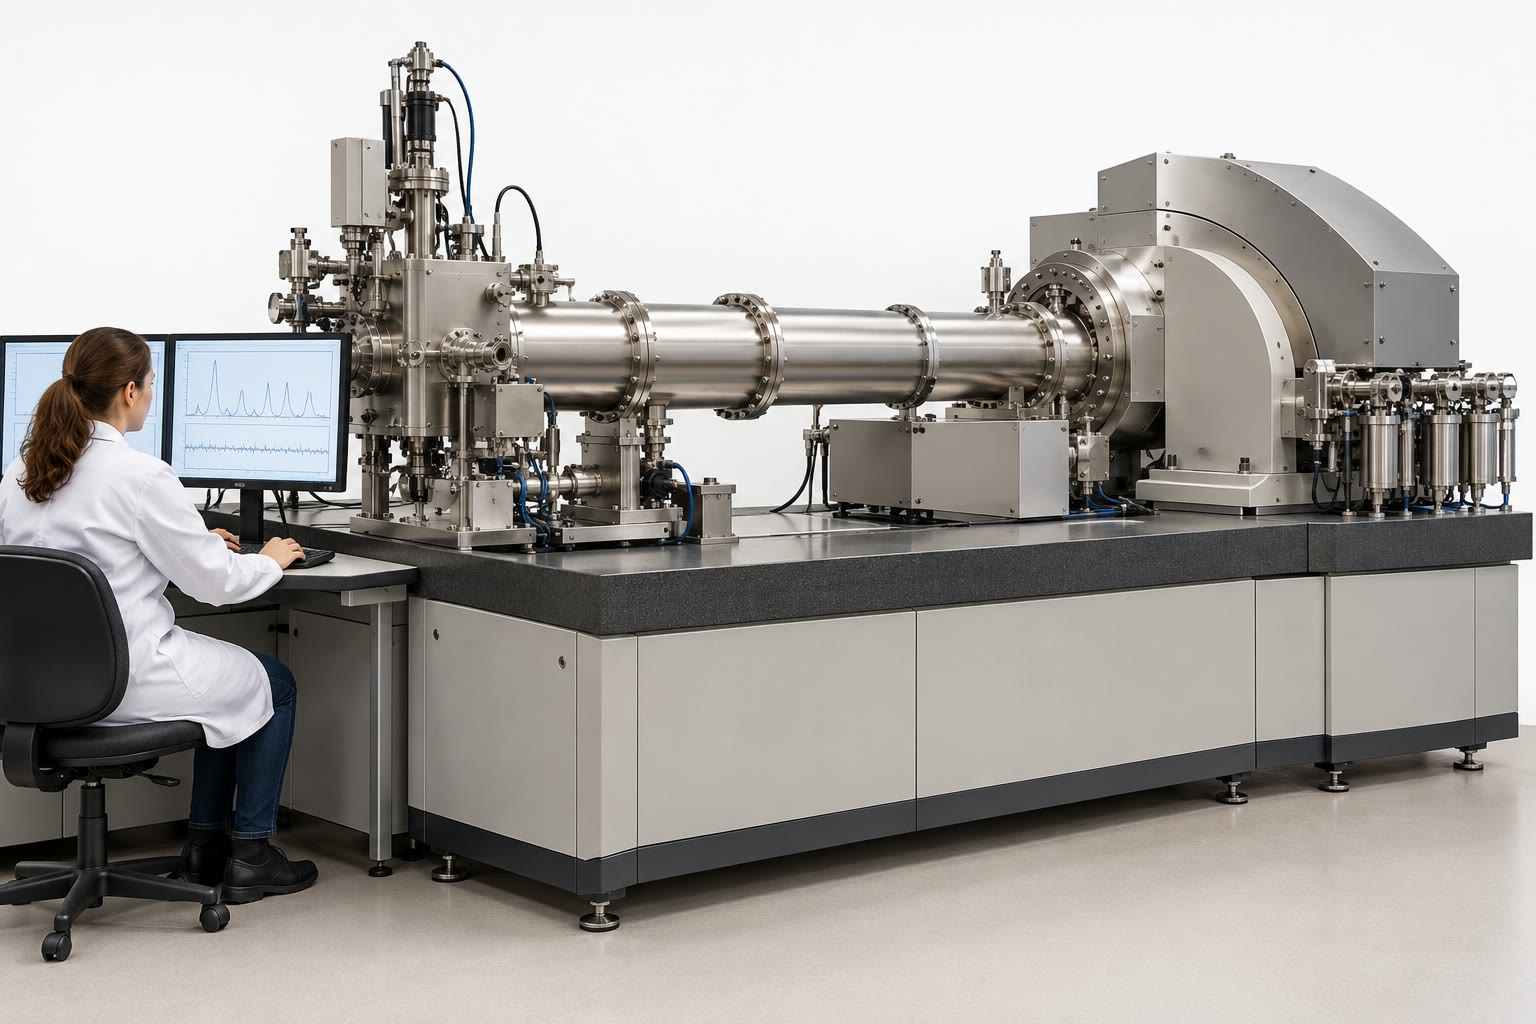
\includegraphics[width=\linewidth]{images/book4/ai/b2-isotope-lab.jpg}
\par\smallskip{\scriptsize Spectromètre de masse multicollecteur dans un laboratoire
d'isotopes. Illustration générée par IA.}
\end{minipage}
\end{inthelab}
% ledger: white:chur

\section{Exercices}

\begin{exercise}[$\star$]\label{exo:b2:isotope-geochemistry:1}
Un basalte de Tristan da Cunha a $^{143}\mathrm{Nd}/^{144}\mathrm{Nd} = 0.51249$ et
un de Mangaia, 0.51285. Calculer leurs $\varepsilon_{\mathrm{Nd}}$ et celui du
MORB moyen (0.513074). Quelles sources ont eu un Sm/Nd plus élevé que les \omterm{def:b2:planet-formation-meteorites:chondrule}{chondrites}~?
\end{exercise}

\begin{exercise}[$\star$]\label{exo:b2:isotope-geochemistry:2}
Le rapport $^{18}\mathrm{O}/^{16}\mathrm{O}$ vaut \num{2.0052e-3} dans le \omterm{def:b2:isotope-geochemistry:standards}{VSMOW} et
\num{2.0672e-3} dans le \omterm{def:b2:isotope-geochemistry:standards}{VPDB}. Quel est le $\delta^{18}\mathrm{O}$ du \omterm{def:b2:isotope-geochemistry:standards}{VPDB} sur l'échelle \omterm{def:b2:isotope-geochemistry:standards}{VSMOW}~?
Une calcite a $\delta^{18}\mathrm{O} = -2.0$ pour mille (\omterm{def:b2:isotope-geochemistry:standards}{VPDB})~; calculer son rapport
et son $\delta^{18}\mathrm{O}$ sur l'échelle \omterm{def:b2:isotope-geochemistry:standards}{VSMOW}.
\end{exercise}

\begin{exercise}[$\star$]\label{exo:b2:isotope-geochemistry:3}
Calculer le $^{143}\mathrm{Nd}/^{144}\mathrm{Nd}$ du CHUR il y a \qty{1.0}{Ga} et
il y a \qty{4.567}{Ga} ($\lambda_{147} = \qty{6.524e-12}{\per\year}$,
$^{147}\mathrm{Sm}/^{144}\mathrm{Nd} = 0.1966$, aujourd'hui 0.512638).
\end{exercise}

\begin{exercise}[$\star$]\label{exo:b2:isotope-geochemistry:4}
Un échantillon de neige d'une station de montagne a $\delta^{18}\mathrm{O} = -18.0$ pour mille.
Quel $\delta\mathrm{D}$ prédit la \omterm{prop:b2:isotope-geochemistry:mwl}{droite des eaux météoriques}~? Une eau de lac a
$\delta^{18}\mathrm{O} = -4.0$ et $\delta\mathrm{D} = -42$ pour mille~: calculer son excès en deutérium
$d = \delta\mathrm{D} - 8\delta^{18}\mathrm{O}$, et dire si elle se situe au-dessus ou
au-dessous de la droite.
\end{exercise}

\begin{exercise}[$\star\star$]\label{exo:b2:isotope-geochemistry:5}
Évaluer $Q$ de la proposition de croissance linéaire. Un granite a Sm \qty{6.0}{ppm}
et Nd \qty{30}{ppm} (CI~: 0.145 et \qty{0.457}{ppm}). Calculer son
$f_{\mathrm{Sm/Nd}}$, ainsi que la variation de son $\varepsilon_{\mathrm{Nd}}$ sur
\qty{500}{Ma}.
\end{exercise}

\begin{exercise}[$\star\star$]\label{exo:b2:isotope-geochemistry:6}
Une croûte séparée il y a \qty{2.7}{Ga} d'un manteau dont
$\varepsilon_{\mathrm{Nd}} = +3.5$, avec $f_{\mathrm{Sm/Nd}} = -0.45$. Estimer son
$\varepsilon_{\mathrm{Nd}}$ actuel à l'aide de la proposition de croissance linéaire. Le calcul
exact donne $-27.3$~; de combien l'approximation diffère-t-elle, et pourquoi est-elle
trop élevée ou trop basse~?
\end{exercise}

\begin{exercise}[$\star\star$]\label{exo:b2:isotope-geochemistry:7}
Un magma basaltique (Sr \qty{130}{ppm}, $^{87}\mathrm{Sr}/^{86}\mathrm{Sr} = 0.7030$)
assimile un granite (Sr \qty{320}{ppm}, 0.7200). Calculer
le $^{87}\mathrm{Sr}/^{86}\mathrm{Sr}$ de mélanges à 5, 10 et 20 pour cent de granite.
Montrer que $^{87}\mathrm{Sr}/^{86}\mathrm{Sr}$ est une droite en fonction de $1/\mathrm{Sr}$
et donner sa pente et son ordonnée à l'origine.
\end{exercise}

\begin{exercise}[$\star\star$]\label{exo:b2:isotope-geochemistry:8}
Avec les facteurs de fractionnement liquide--vapeur 1.0098 ($^{18}$O) et 1.084 (D) à
\qty{20}{\degreeCelsius}, calculer le $\delta^{18}\mathrm{O}$ et le $\delta\mathrm{D}$ d'une
vapeur en équilibre avec de l'eau de mer (0, 0), ainsi que la pente
$\delta\mathrm{D}/\delta^{18}\mathrm{O}$ de la droite joignant l'eau à la vapeur. Refaire le calcul
à \qty{0}{\degreeCelsius} (1.0117 et 1.111). Comparer avec la \omterm{prop:b2:isotope-geochemistry:mwl}{droite des eaux météoriques}.
\end{exercise}

\begin{exercise}[$\star\star$]\label{exo:b2:isotope-geochemistry:9}
La croûte continentale représente 0.51 pour cent de la masse de la Terre silicatée et contient,
en moyenne, \qty{27}{ppm} de Nd contre \qty{1.25}{ppm} pour la Terre silicatée. Prendre
l'$\varepsilon_{\mathrm{Nd}}$ de la croûte égal à $-15$ et celui de la Terre silicatée à 0. Quelle
part du néodyme la croûte détient-elle~? Si le reste du manteau était uniforme,
quelle serait son $\varepsilon_{\mathrm{Nd}}$~? Quelle part du néodyme doit détenir un
réservoir appauvri à $+8.5$ si le reste du manteau est chondritique~?
\end{exercise}

\begin{exercise}[$\star\star\star$]\label{exo:b2:isotope-geochemistry:10}
Montrer que, dans la proposition de croissance linéaire, les termes négligés sont de taille relative
d'environ $\lambda t/2$. Sur l'âge de la Terre, quelle est cette valeur, et quelle
erreur cela introduit-il dans $\varepsilon_{\mathrm{Nd}}$ pour $f = -0.45$ sur
\qty{2.7}{Ga}~?
\end{exercise}

\begin{exercise}[$\star\star\star$]\label{exo:b2:isotope-geochemistry:11}
Deux constituants ont des rapports Sr/Nd de 13.3 (A) et 5.0 (B). En utilisant la démonstration de
l'\omterm{prop:b2:isotope-geochemistry:mixing}{hyperbole de mélange}, trouver la part $s'$ du strontium provenant de A dans un mélange où A
fournit une part $s = 0.5$ du néodyme. Pour quelle valeur de $s$ les deux
parts diffèrent-elles le plus~?
\end{exercise}

\begin{exercise}[$\star\star\star$]\label{exo:b2:isotope-geochemistry:12}
Un modèle en boîtes donne 2.3 à 2.6 fois le volume actuel de croûte continentale,
\qty{7.2e9}{km^3}, généré depuis la formation de la Terre il y a \qty{4.5}{Ga}, et 1.3 à 1.6
fois détruit. Calculer les taux moyens de production et de destruction en
\unit{km^3} par an. Comparer-les aux taux actuels des zones de subduction,
\qty{2.7}{km^3} par an ajoutés et \qty{3.2}{km^3} par an retirés.
\end{exercise}

\section{Problème~: trois îles, trois manteaux}

\begin{problem}[{Problème du week-end --- placer les laves de trois îles sur la
bande mantellique, séparer un mélange d'un troisième constituant, et dater le
sédiment recyclé}]
\label{pb:b2:isotope-geochemistry:1}
Trois îles volcaniques d'un océan imaginaire, Kora, Vel et Asha, émettent des basaltes
aux rapports isotopiques ci-dessous. Un géochimiste modélise leurs sources avec deux
constituants~: un \omterm{def:b2:isotope-geochemistry:reservoirs}{manteau appauvri} semblable à la source du MORB (Sr \qty{10}{ppm}, Nd
\qty{0.75}{ppm}, $^{87}\mathrm{Sr}/^{86}\mathrm{Sr} = 0.70282$,
$^{143}\mathrm{Nd}/^{144}\mathrm{Nd} = 0.51307$) et un vieux sédiment renvoyé dans le
manteau par subduction (Sr \qty{200}{ppm}, Nd \qty{40}{ppm}, $0.72000$, $0.51141$~;
$^{147}\mathrm{Sm}/^{144}\mathrm{Nd} = 0.110$, $^{87}\mathrm{Rb}/^{86}\mathrm{Sr} = 0.50$).
Kora~: $0.70410$, $0.51278$~; Vel~: $0.70618$, $0.51242$~; Asha~: $0.70290$, $0.51288$
($^{87}\mathrm{Sr}/^{86}\mathrm{Sr}$, $^{143}\mathrm{Nd}/^{144}\mathrm{Nd}$). CHUR aujourd'hui~:
$^{143}\mathrm{Nd}/^{144}\mathrm{Nd} = 0.512638$, $^{147}\mathrm{Sm}/^{144}\mathrm{Nd} =
0.1966$~; $\lambda_{147} = \qty{6.524e-12}{\per\year}$, $\lambda_{87} =
\qty{1.3972e-11}{\per\year}$.

\medskip\noindent\textbf{Partie I --- Placer les îles.}
\begin{enumerate}
\item Calculer $\varepsilon_{\mathrm{Nd}}$ des deux constituants.
\item Calculer $\varepsilon_{\mathrm{Nd}}$ des trois îles.
\item Placer les cinq compositions sur un diagramme Sr--$\varepsilon_{\mathrm{Nd}}$. Quelles
îles se situent du côté enrichi du CHUR~?
\item Asha a presque le rapport du strontium du \omterm{def:b2:isotope-geochemistry:reservoirs}{manteau appauvri}, mais un $\varepsilon_{\mathrm{Nd}}$
beaucoup plus bas. Où se place-t-il par rapport à la bande mantellique, et à quel groupe
d'îles du chapitre ressemble-t-il~?
\item Pourquoi peut-on prendre les rapports isotopiques des laves pour ceux de leurs sources,
bien que les laves aient des rapports Sm/Nd et Rb/Sr très différents de ceux de leurs sources~?
\item Une lave de Kora de $^{147}\mathrm{Sm}/^{144}\mathrm{Nd} = 0.12$ est âgée de \qty{1}{Ma}.
De combien son $^{143}\mathrm{Nd}/^{144}\mathrm{Nd}$ a-t-il augmenté depuis l'éruption, en
unités epsilon~? Cela a-t-il de l'importance~?
\end{enumerate}

\noindent\textbf{Partie II --- Le mélange des deux constituants.}
\begin{enumerate}[resume]
\item Écrire la concentration en néodyme et le $^{143}\mathrm{Nd}/^{144}\mathrm{Nd}$ d'un
mélange de fraction massique $f$ de sédiment.
\item Calculer $\varepsilon_{\mathrm{Nd}}$ de mélanges avec $f = 0.5$, 1, 2 et 5 pour
cent.
\item Calculer le $^{87}\mathrm{Sr}/^{86}\mathrm{Sr}$ des mêmes mélanges.
\item Montrer que le $^{87}\mathrm{Sr}/^{86}\mathrm{Sr}$ des mélanges est une droite
en fonction de $1/\mathrm{Sr}$, et en donner la pente.
\item Calculer $K = (\mathrm{Sr}/\mathrm{Nd})_{\text{manteau}}/(\mathrm{Sr}/\mathrm{Nd})_{\text{sédiment}}$.
Quel rapport, Sr ou Nd, se rapproche du sédiment le plus vite quand $f$ augmente~?
\item De combien de fois le sédiment est-il plus riche que le manteau en Nd, et en Sr~?
Expliquer avec ces nombres pourquoi un pour cent de sédiment déplace
$\varepsilon_{\mathrm{Nd}}$ d'environ 11 unités.
\item Quelle part du néodyme d'un mélange à $f = 1$ pour cent provient du
sédiment~?
\end{enumerate}

\noindent\textbf{Partie III --- Quelle quantité de sédiment~?}
\begin{enumerate}[resume]
\item Résoudre l'équation de mélange du néodyme pour $f$, connaissant le rapport $R$ du mélange.
\item Calculer $f$ pour Kora à partir de son néodyme.
\item Calculer $f$ pour Kora à partir de son strontium. Les deux résultats concordent-ils~?
\item Calculer $f$ pour Vel à partir de son néodyme et à partir de son strontium.
\item Calculer $f$ pour Asha à partir de son néodyme, puis le rapport du strontium que
ce $f$ prédit. Comparer à la valeur mesurée~: que conclure sur la
source d'Asha~?
\item Suggérer une troisième composante pour Asha, parmi celles du chapitre, et les
rapports parent--fils qu'elle doit avoir eus.
\end{enumerate}

\noindent\textbf{Partie IV --- L'âge du sédiment.}
\begin{enumerate}[resume]
\item Le sédiment a été subduit il y a \qty{2.0}{Ga} et est resté fermé depuis.
Calculer son $^{143}\mathrm{Nd}/^{144}\mathrm{Nd}$, celui du CHUR et son
$\varepsilon_{\mathrm{Nd}}$ à cette époque.
\item Refaire le calcul avec la proposition de croissance linéaire.
\item Calculer le $^{87}\mathrm{Sr}/^{86}\mathrm{Sr}$ du sédiment il y a \qty{2.0}{Ga}.
\item Il y a \qty{2.0}{Ga}, la croûte de la figure en $\varepsilon_{\mathrm{Nd}}$ avait
$\varepsilon_{\mathrm{Nd}} \approx -4.7$. La valeur du sédiment au moment de la subduction est-elle compatible
avec une origine par érosion d'une croûte continentale aussi jeune~?
\item Donner la fraction massique de sédiment recyclé dans la source de l'île la plus
enrichie, nombre clé de ce problème.
\end{enumerate}
\end{problem}
% ledger: white:chur, villa20:sm147, villa22:rb87, gale13:isotopes
